\documentclass[a4paper,12pt]{book}
\usepackage[utf8]{inputenc}

\usepackage{rachwidgets}


\newcommand{\laClass}       {CS 211}
\newcommand{\laSemester}    {Spring 2018}
\newcommand{\laChapter}     {7.4}
\newcommand{\laType}        {Exercise}
\newcommand{\laPoints}      {5}
\newcommand{\laTitle}       {Connections to Matrices and Relations}
\newcommand{\laDate}        {}
\setcounter{chapter}{7}
\setcounter{section}{4}
\addtocounter{section}{-1}
\newcounter{question}

\toggletrue{answerkey}


\title{}
\author{Rachel Singh}
\date{\today}

\pagestyle{fancy}
\fancyhf{}

\lhead{\laClass, \laSemester, \laDate}

\chead{}

\rhead{\laChapter\ \laType\ \iftoggle{answerkey}{ KEY }{}}

\rfoot{\thepage\ of \pageref{LastPage}}

\lfoot{\scriptsize By Rachel Singh, last updated \today}

\renewcommand{\headrulewidth}{2pt}
\renewcommand{\footrulewidth}{1pt}

\begin{document}




\footnotesize
~\\ 
\textbf{\laChapter\ \laType: } In-class exercises are meant to introduce you to a new topic
and provide some practice with the new topic. Work in a team of up to 4 people to complete this exercise.
You can work simultaneously on the problems, or work separate and then check your answers with each other.
Completion score is given for this assignment.

~\\
Team:\\
(1) \tab[6cm] (2) \\
(3) \tab[6cm] (4)

\hrulefill
\normalsize 



% KEY ------------------------------------ %

\begin{enumerate}

    \item   
        \begin{tikzpicture}
            \filldraw (-7,1) circle (1pt) node[left] {1};
            \filldraw (-7,2) circle (1pt) node[left] {2};
            \filldraw (-6,3) circle (1pt) node[above] {3};
            \filldraw (-5,1) circle (1pt) node[right] {5};
            \filldraw (-5,2) circle (1pt) node[right] {4};

            \draw (-7,1) -- (-5,1);
            \draw (-7,1) -- (-7,2);
            \draw (-7,2) -- (-5,2);
            \draw (-7,2) -- (-6,3);
            \draw (-7,1) to[bend right] (-5,1);
            \draw (-4.7,2) circle (10pt);
            
            \node[above,rotate=90] at (-0.5, 2) {Rows};
            \node[left] at (0,4) {1};
            \node[left] at (0,3) {2};
            \node[left] at (0,2) {3};
            \node[left] at (0,1) {4};
            \node[left] at (0,0) {5};
            \node[above] at (3,5) {Columns};
            \node[above] at (1,4.5) {1};
            \node[above] at (2,4.5) {2};
            \node[above] at (3,4.5) {3};
            \node[above] at (4,4.5) {4};
            \node[above] at (5,4.5) {5};
            \draw (0.5,-0.5) -- (0,-0.5) -- (0,4.5) -- (0.5,4.5);
            \draw (5.5,-0.5) -- (6,-0.5) -- (6,4.5) -- (5.5,4.5);

            \solution{ \node at (1,0) {2}; }{}
            \solution{ \node at (2,0) {0}; }{}
            \solution{ \node at (3,0) {0}; }{}
            \solution{ \node at (4,0) {0}; }{}
            \solution{ \node at (5,0) {0}; }{}
            
            \solution{ \node at (1,1) {0}; }{}
            \solution{ \node at (2,1) {1}; }{}
            \solution{ \node at (3,1) {0}; }{}
            \solution{ \node at (4,1) {1}; }{}
            \solution{ \node at (5,1) {0}; }{}
            
            \solution{ \node at (1,2) {0}; }{}
            \solution{ \node at (2,2) {1}; }{}
            \solution{ \node at (3,2) {0}; }{}
            \solution{ \node at (4,2) {0}; }{}
            \solution{ \node at (5,2) {0}; }{}
            
            \solution{ \node at (1,3) {1}; }{}
            \solution{ \node at (2,3) {0}; }{}
            \solution{ \node at (3,3) {1}; }{}
            \solution{ \node at (4,3) {1}; }{}
            \solution{ \node at (5,3) {0}; }{}
            
            \solution{ \node at (1,4) {0}; }{}
            \solution{ \node at (2,4) {1}; }{}
            \solution{ \node at (3,4) {0}; }{}
            \solution{ \node at (4,4) {0}; }{}
            \solution{ \node at (5,4) {2}; }{}
        \end{tikzpicture}

    \hrulefill

    \item 
        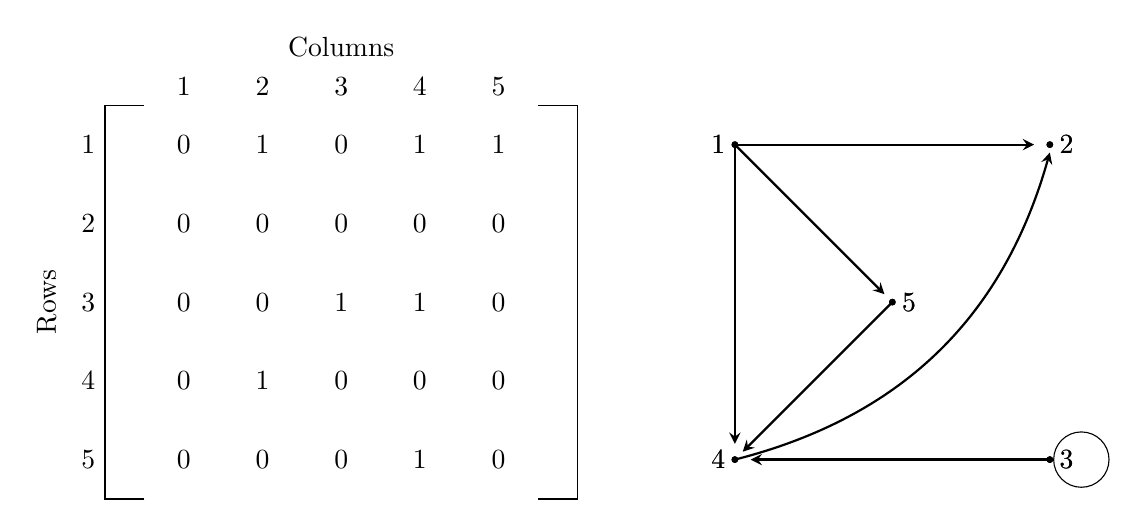
\begin{tikzpicture}[arrow/.style = {thick,-stealth}]
            \node[above,rotate=90] at (-0.5, 2) {Rows};
            \node[left] at (0,4) {1};
            \node[left] at (0,3) {2};
            \node[left] at (0,2) {3};
            \node[left] at (0,1) {4};
            \node[left] at (0,0) {5};
            \node[above] at (3,5) {Columns};
            \node[above] at (1,4.5) {1};
            \node[above] at (2,4.5) {2};
            \node[above] at (3,4.5) {3};
            \node[above] at (4,4.5) {4};
            \node[above] at (5,4.5) {5};
            \draw (0.5,-0.5) -- (0,-0.5) -- (0,4.5) -- (0.5,4.5);
            \draw (5.5,-0.5) -- (6,-0.5) -- (6,4.5) -- (5.5,4.5);

            \node at (1,0) {0};
            \node at (2,0) {0};
            \node at (3,0) {0};
            \node at (4,0) {1};
            \node at (5,0) {0};
            
            \node at (1,1) {0};
            \node at (2,1) {1};
            \node at (3,1) {0};
            \node at (4,1) {0};
            \node at (5,1) {0};
            
            \node at (1,2) {0};
            \node at (2,2) {0};
            \node at (3,2) {1};
            \node at (4,2) {1};
            \node at (5,2) {0};
            
            \node at (1,3) {0};
            \node at (2,3) {0};
            \node at (3,3) {0};
            \node at (4,3) {0};
            \node at (5,3) {0};
            
            \node at (1,4) {0};
            \node at (2,4) {1};
            \node at (3,4) {0};
            \node at (4,4) {1};
            \node at (5,4) {1};

            \solution{
                \filldraw (8, 0)  circle (1pt) node[left]    {4};
                \filldraw (12,0)  circle (1pt) node[right]   {3};
                \filldraw (8, 4)  circle (1pt) node[left]    {1};
                \filldraw (12,4)  circle (1pt) node[right]   {2};
                \filldraw (10,2)  circle (1pt) node[right]   {5};

                \draw[arrow] (8,4)  -- (8,0.2);
                \draw[arrow] (8,4)  -- (9.9, 2.1);
                \draw[arrow] (10,2) -- (8.1,0.1);
                \draw[arrow] (8,4)  -- (11.8,4);
                \draw[arrow] (12,0) -- (8.2,0);
                \draw (12.4,0) circle (10pt);
                \draw[arrow] (8,0) to[bend right] (12,3.9);
            }{
                \filldraw (8, 0)  circle (1pt) node[left]    {4};
                \filldraw (12,0)  circle (1pt) node[right]   {3};
                \filldraw (8, 4)  circle (1pt) node[left]    {1};
                \filldraw (12,4)  circle (1pt) node[right]   {2};
                \filldraw (10,2)  circle (1pt) node[right]   {5};
            }
        \end{tikzpicture}

    \hrulefill

    \item   
        \solution{
            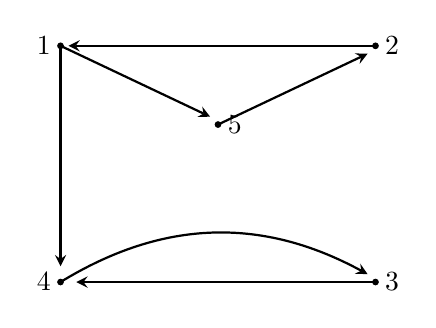
\begin{tikzpicture}[arrow/.style = {thick,-stealth}]
                \filldraw (8, 0)  circle (1pt) node[left]    {4};
                \filldraw (12,0)  circle (1pt) node[right]   {3};
                \filldraw (8, 3)  circle (1pt) node[left]    {1};
                \filldraw (12,3)  circle (1pt) node[right]   {2};
                \filldraw (10,2)  circle (1pt) node[right]   {5};

                \draw[arrow] (8,3)  -- (8,0.2);
                \draw[arrow] (8,3)  -- (9.9, 2.1);
                \draw[arrow] (10,2) -- (11.9,2.9);
                \draw[arrow] (12,3)  -- (8.1,3);
                \draw[arrow] (12,0) -- (8.2,0);
                \draw[arrow] (8,0) to[bend left] (11.9,0.1);
            \end{tikzpicture}
            
        }{
            \begin{center}
                \begin{tikzpicture}
                    \filldraw (8, 0)  circle (1pt) node[left]    {4};
                    \filldraw (12,0)  circle (1pt) node[right]   {3};
                    \filldraw (8, 3)  circle (1pt) node[left]    {1};
                    \filldraw (12,3)  circle (1pt) node[right]   {2};
                    \filldraw (10,1.5)  circle (1pt) node[right]   {5};
                \end{tikzpicture}
            \end{center}
        }

\end{enumerate}




\end{document}

